\ifspanish

\question Se tiene un problema de decisión binaria definido por las verosimilitudes representadas en la siguiente figura:
\begin{center}
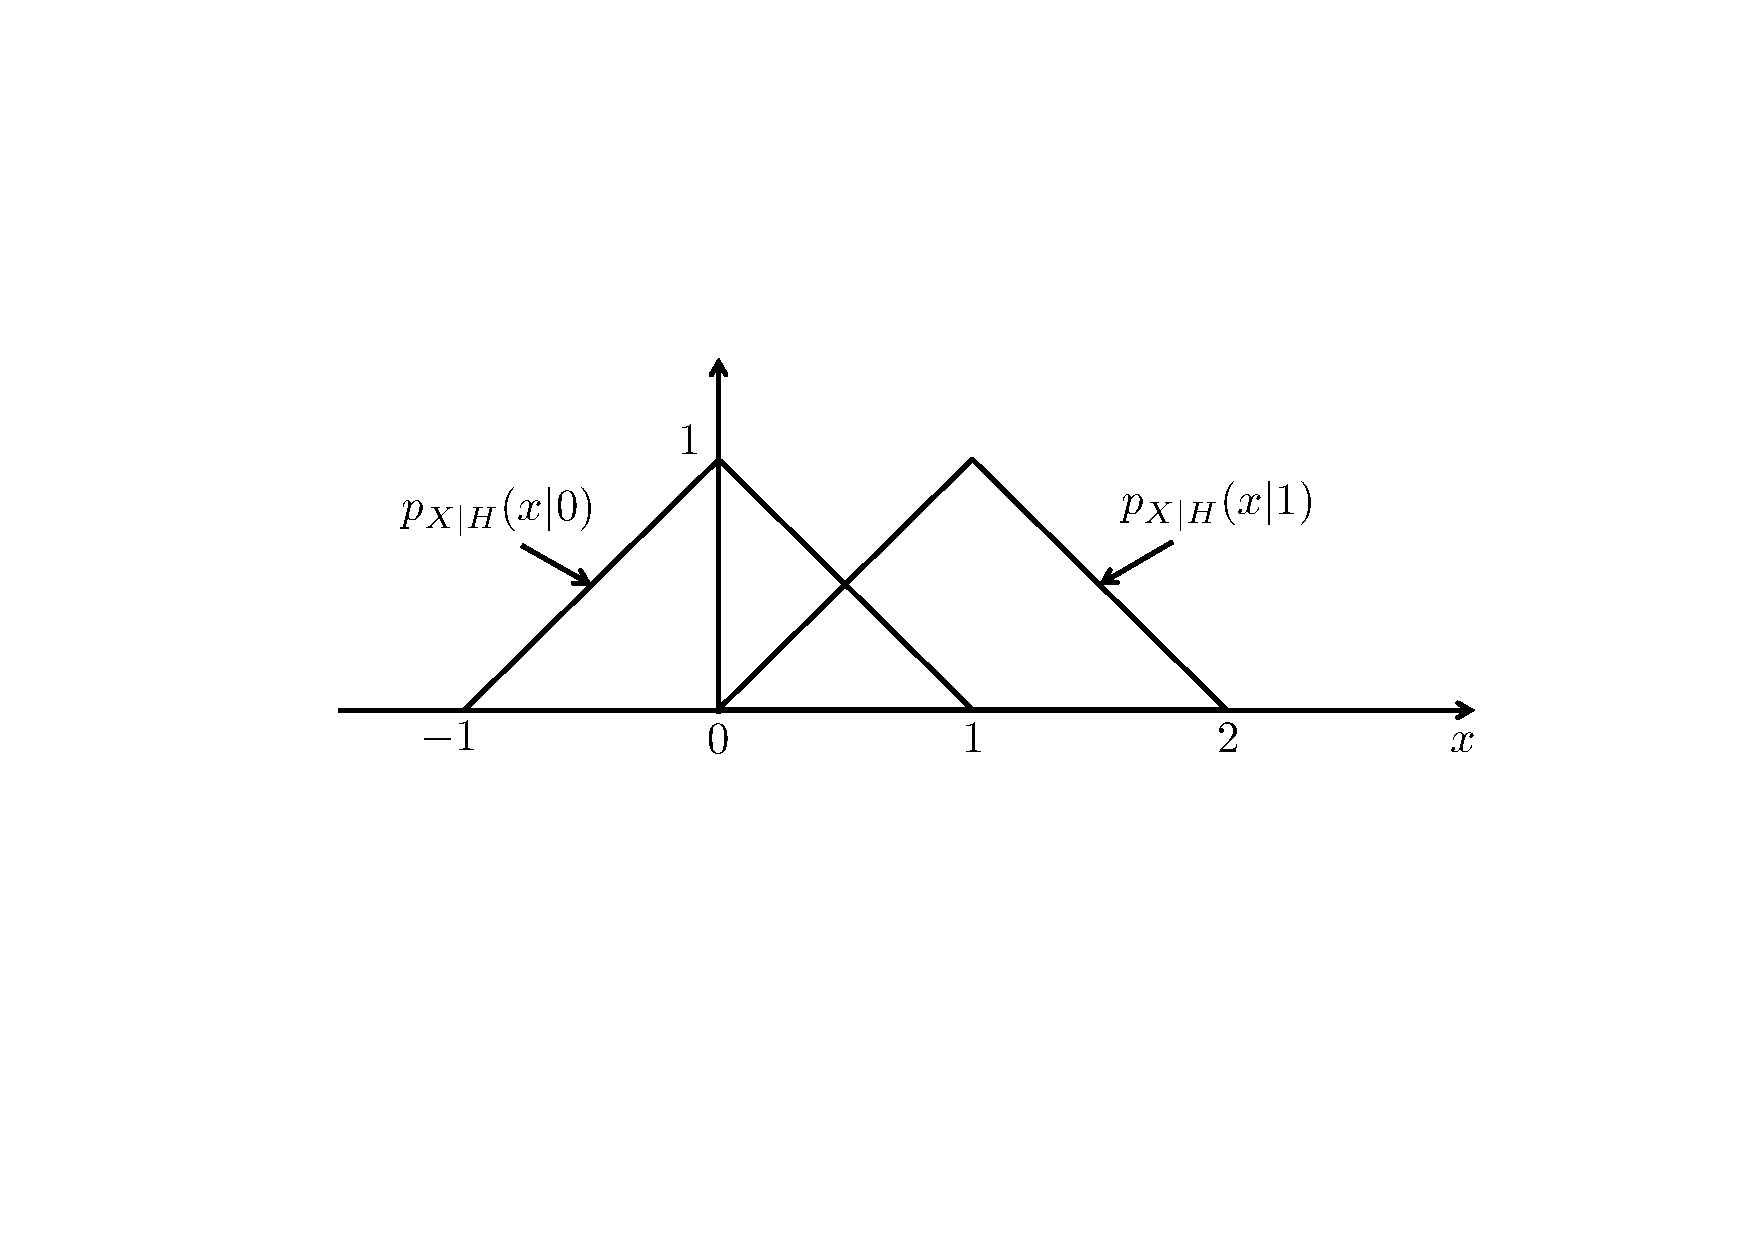
\includegraphics[scale=0.45]{Figuras/Fig_prob_dec.pdf}
\end{center}
\begin{parts}
\part Obtenga una expresión para las regiones de decisión de un decisor LRT genérico.
\part Obtenga las probabilidades de falsa alarma y de pérdida y represente la curva ROC.
\end{parts}

\begin{solution}
\begin{parts}
\part $ \left \{
  \begin{array}{ll}
-1 \le x \le 0    & D=0 \\
0 \le x \le 1    & x \dunodcero \displaystyle \frac{\eta}{1+\eta}=\nu \\
1 \le x \le 2    & D=1 \\
  \end{array}
\right.$

\part 
$ \left \{
  \begin{array}{ll}
-1 \le \nu \le 0    &  \pmis=0 \\
0<\nu<1    & \pfa=\frac{1}{2}\left(1-\nu \right) ^2 \quad \pmis=\frac{1}{2} \nu^2 \\
1 \le \nu \le 2    & \pfa=0 \\
  \end{array}
\right.$

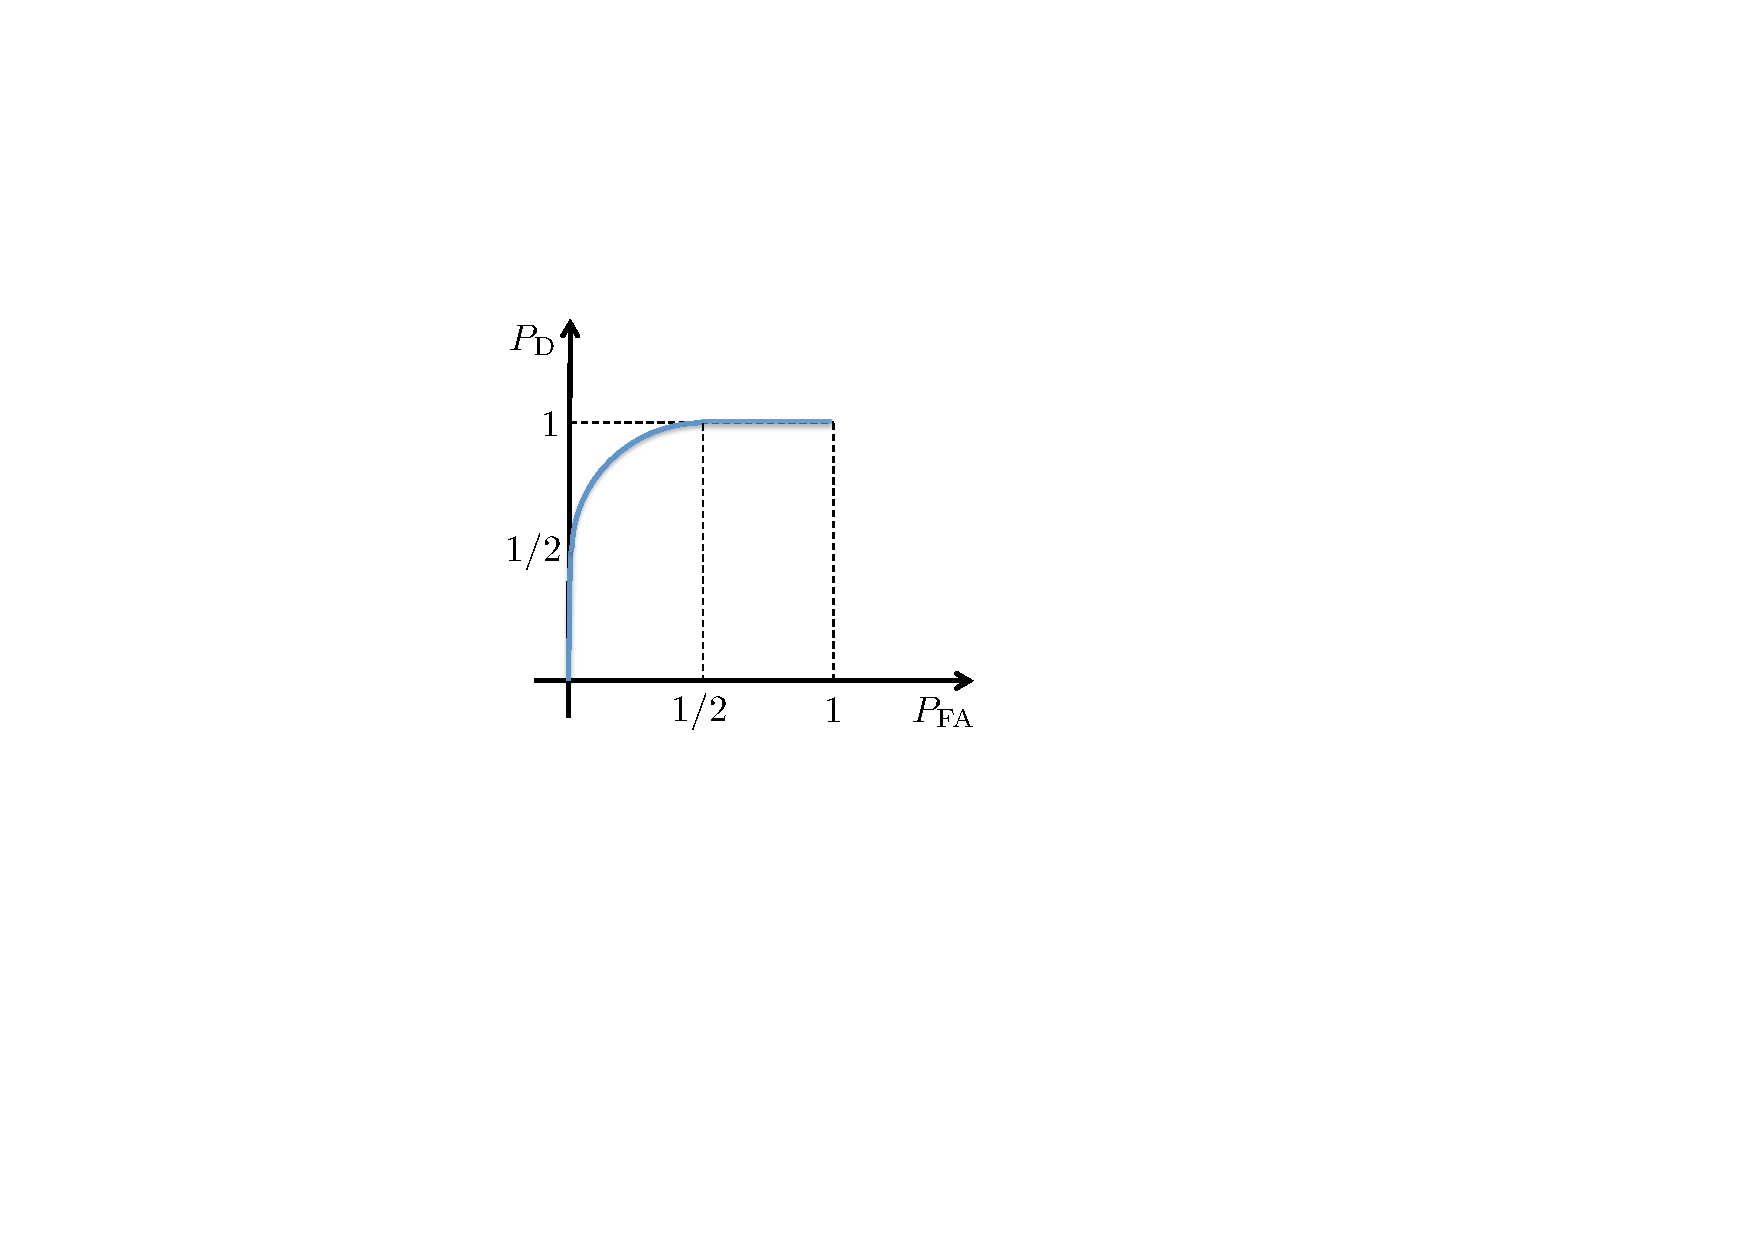
\includegraphics[scale=0.5]{Figuras/ROC_JUN2012}
\end{parts}

\end{solution}

\else

\question We have a binary decision problem characterized by the likelihoods depicted in the following figure:
\begin{center}
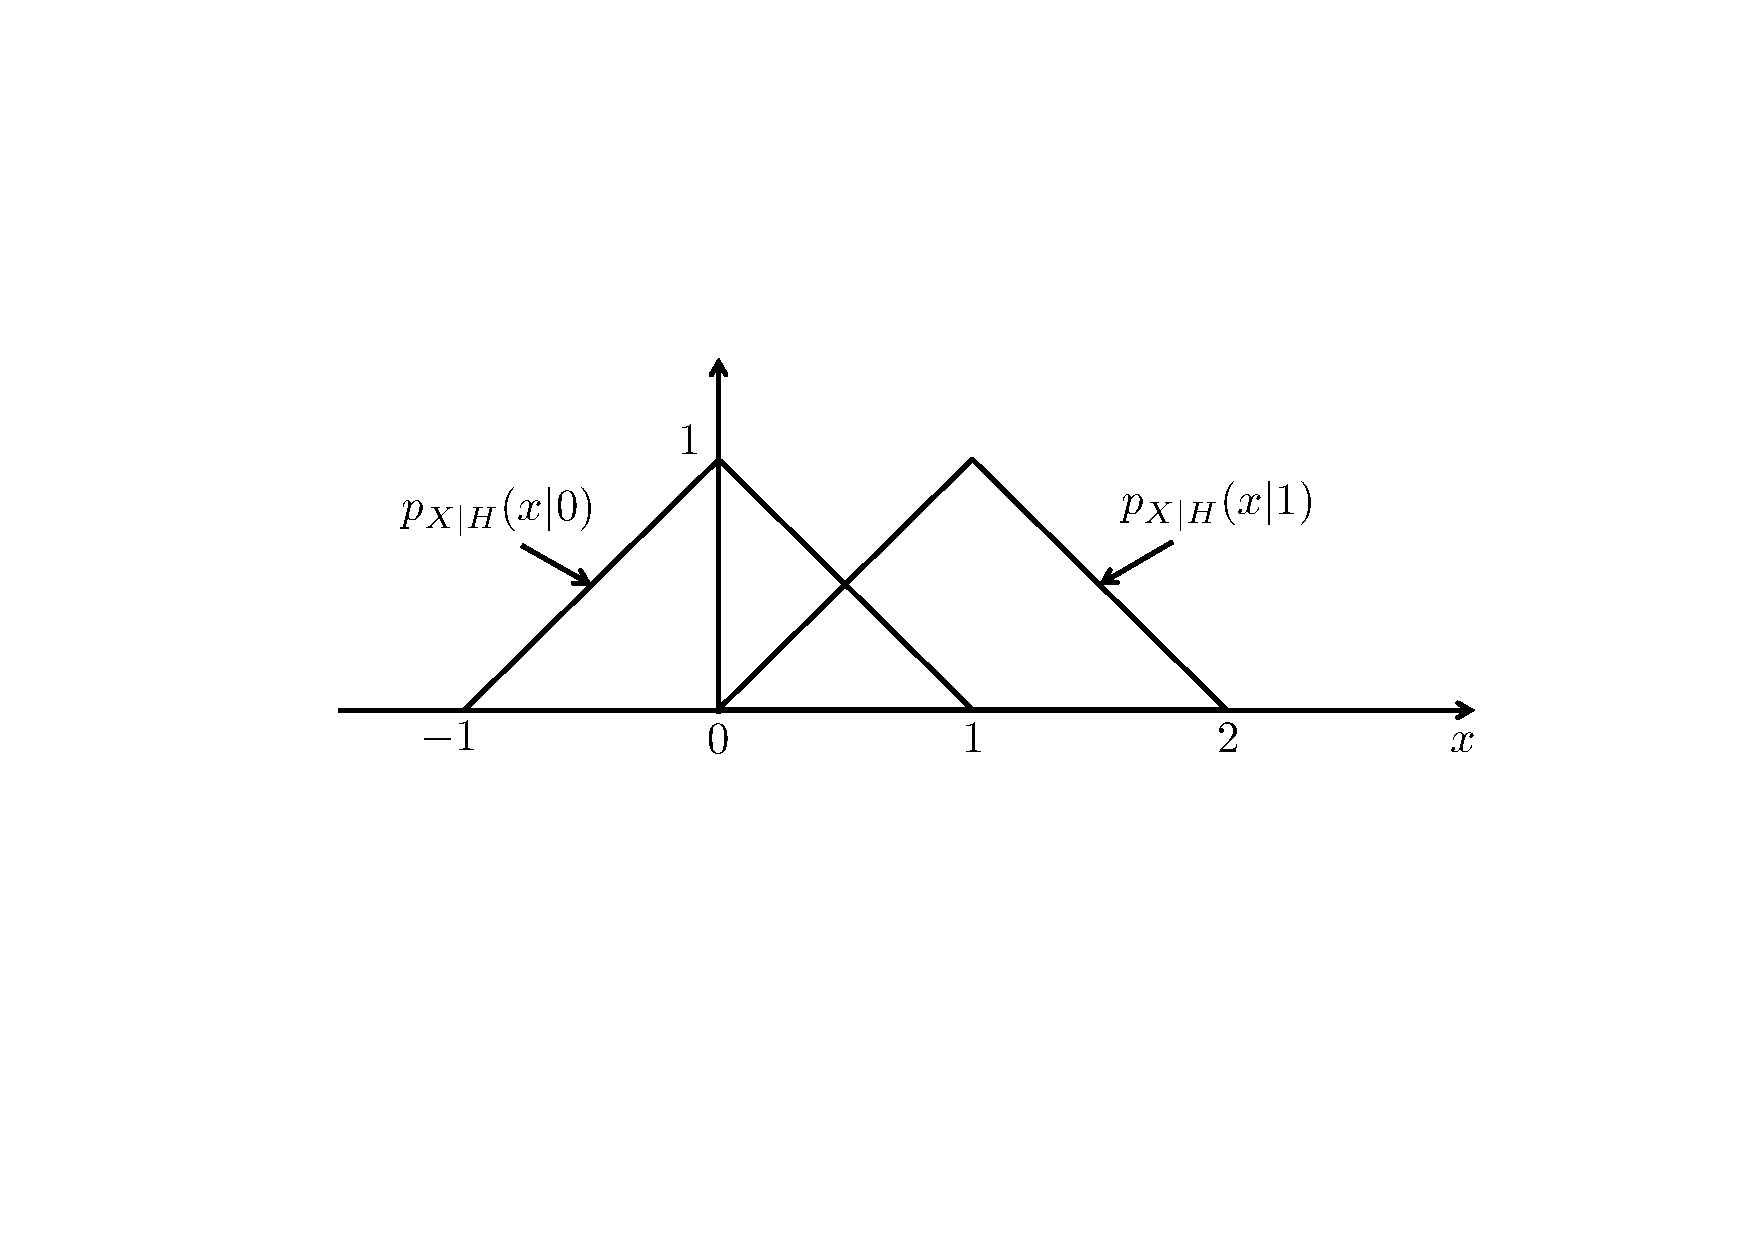
\includegraphics[scale=0.45]{Figuras/Fig_prob_dec.pdf}
\end{center}
\begin{parts}
\part Find an analytical expression for the decision regions of a generic LRT.
\part Obtain the probabilities of false alarm and missing, and plot the ROC curve.
\end{parts}

\begin{solution}
\begin{parts}
\part $ \left \{
  \begin{array}{ll}
-1 \le x \le 0    & D=0 \\
0 \le x \le 1    & x \dunodcero \displaystyle \frac{\eta}{1+\eta}=\nu \\
1 \le x \le 2    & D=1 \\
  \end{array}
\right.$

\part 
$ \left \{
  \begin{array}{ll}
-1 \le \nu \le 0    &  \pmis=0 \\
0<\nu<1    & \pfa=\frac{1}{2}\left(1-\nu \right) ^2 \quad \pmis=\frac{1}{2} \nu^2 \\
1 \le \nu \le 2    & \pfa=0 \\
  \end{array}
\right.$

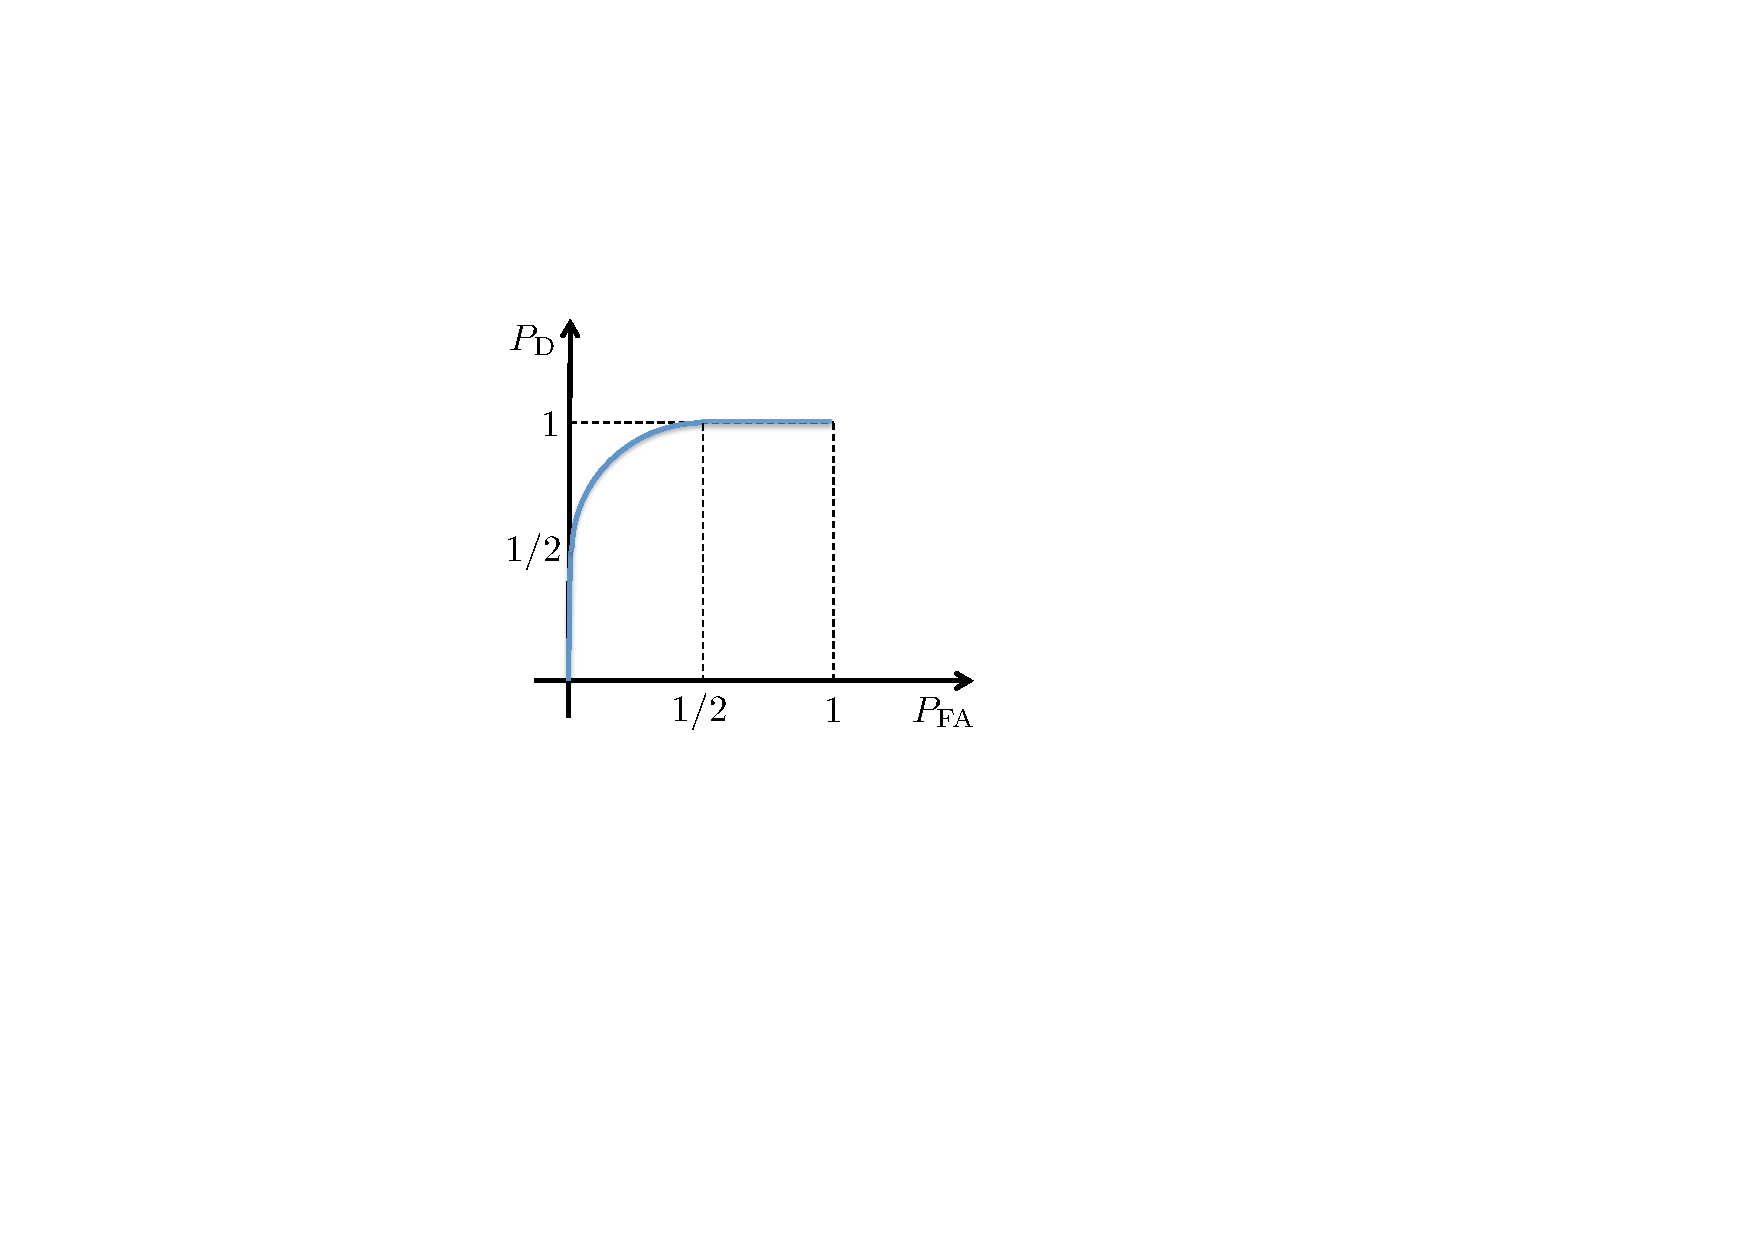
\includegraphics[scale=0.5]{Figuras/ROC_JUN2012}
\end{parts}

\end{solution}

\fi